\subsection{\eigendocs{}}\label{subsubsec:eigendocs}

% this work
\begin{figure}[!htb] % htp = hier (h), top (t), oder auf einer eigenen Seite (p).
    \centering
    \includesvg[width=1.0\textwidth]{images/eigendocs}
    \caption[\eigendocs{} procedure]{From PDFs to \eigendocs{}.
    Firstly, the first page of a document is converted to an image.
    Then, the image is preprocessed:
    It is placed on a white canvas, to ensure all images have the same dimensions.
    Moreover, it is converted to greyscale and normalized to values between zero and one.
    Afterwards, the two-dimensional image is reshaped into a one-dimensional array.
    Lastly, the image is compressed using \eigendocs{}.
    }
    \label{fig:eigendocs_procedure}
\end{figure}

In this work, the \eigenfaces{} approach from \autoref{subsec:eigenface} is used to compress the images of the first page of the documents.
The idea is that documents not only hold textual information but also visual information, such as layout, company logo or signature.
By mapping those images on a subspace, they ought to be grouped by visual similarity.
The procedure of the \eigenfaces{} adaption \textit{\eigendocs{}} is displayed in \autoref{fig:eigendocs_procedure}.
Different stages of this approach are displayed in \autoref{fig:preprocessed_docs_eigendocs}.

\begin{figure}[!htb] % htp = hier (h), top (t), oder auf einer eigenen Seite (p).
    \centering
    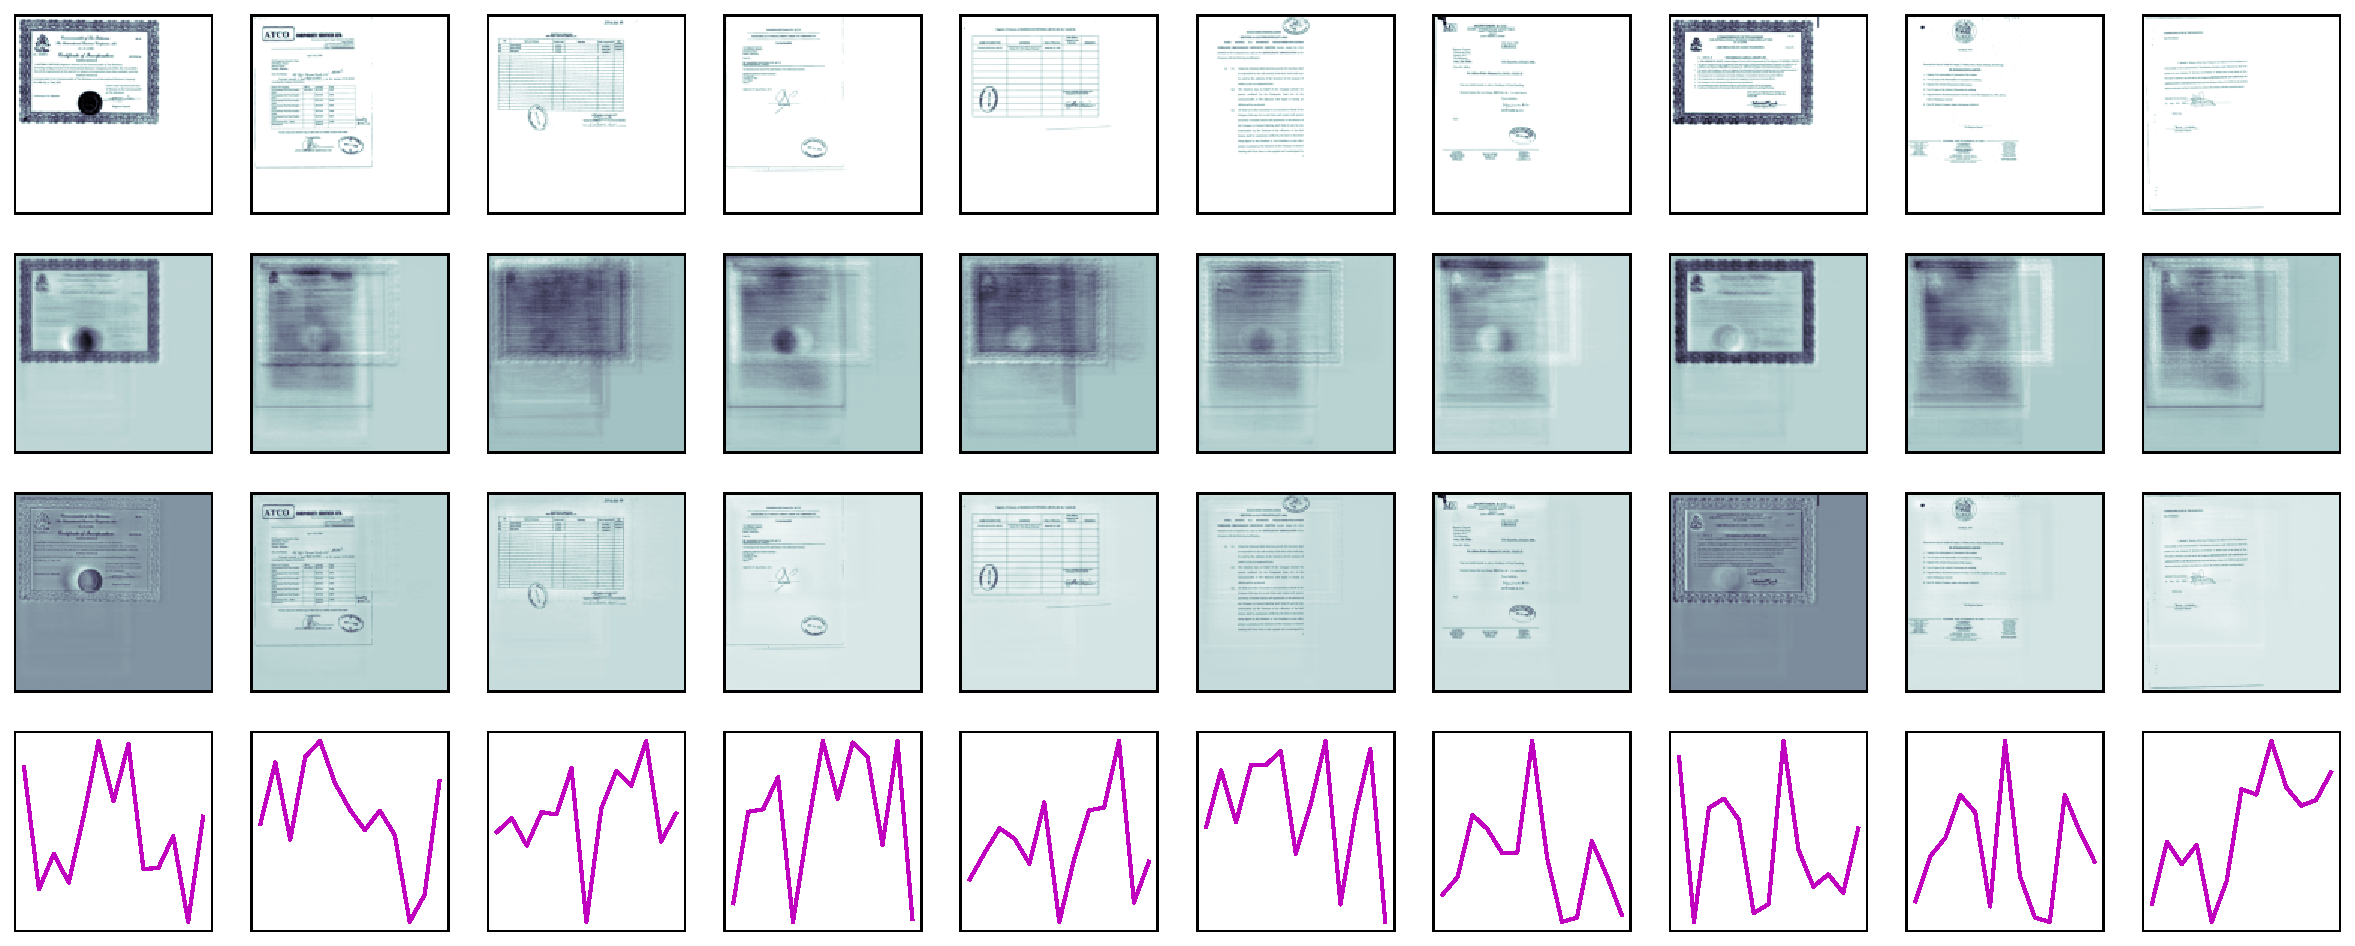
\includegraphics[width=1\textwidth]{images/Eigendocs/transformation/eigendocs.pdf}
    \caption[Preprocessing 10 randomly selected documents from the test set]{10 randomly selected documents from the test set.
    The number of images in the test set is 561, while the \acs*{pca} model is fitted to 1680 training images.
    The original images are displayed in the first row.
    The second row shows the reconstruction from their compressed version in the fourth row.
    The third row shows the reconstruction error, i.e.\ the difference between the reconstructed and the original image.
    The last row presents the greyscale values of the compressed 13-dimensional image as a line.
    }
    \label{fig:preprocessed_docs_eigendocs}
\end{figure}

% procedure
The documents are first read from a directory. 
Subsequently, their first page is converted to an image and saved.
When initially filling the database, these images are read from their directory.
Firstly, the maximum height and width among all images in a corpus of 1000 randomly sampled images are calculated.
The selection of 1000 images is used to reduce the run time of the script.
The maximum height and width are used to create a white canvas for each image which forms the background.
Every image is placed in the upper left corner.
Hence, assuming the selection of documents used to fit the \ac{pca} model is representative, 
scaling is not necessary and thus, the portion of white pixels on the right and bottom side encodes the dimension of the former image.
Therefore, the relative size of images in the corpus is incorporated in the resulting representation of the input images.
However, some images are bigger than the maximum values of the selected images and as a consequence are scaled.

\begin{listing}[htp]
    \begin{minted}[escapeinside=||]{python3}
        def rgb2gray(img):
            return 0.299*img[:,:,0] + 0.587*img[:,:,1] + 0.114*img[:,:,2]
        # more code
        C = np.ones((max_w,max_h))
        C[:doc.shape[0],:doc.shape[1]] = rgb2gray(doc)|\phantomsection\label{line:color}|
        documents.append(C.ravel())|\phantomsection\label{line:ravel}|
    \end{minted}
    \caption[Preprocessing of the input images]{Preprocessing of the input images from \thesissupervisor{}.
    Conversion of RGB pixel values to greyscale according to \cite{RGB2Grey}.
    The background is a white canvas.
    The images are converted to one-dimensional greyscale values.}
    \label{lst:preproc_images}
\end{listing}

Afterwards, the images are converted to greyscale using line \ref{line:color} of \lst{lst:preproc_images}.
Before returning the image, the two-dimensional image vectors are converted to one-dimensional ones as displayed in line \ref{line:ravel} of \lst{lst:preproc_images}.
The decomposition is transformed using \ac{pca} as displayed in \lst{lst:pca_svd}.
The implementation of \ac{pca} from \href{https://scikit-learn.org/stable/modules/generated/sklearn.decomposition.PCA.html}{sklearn} 
intrinsically normalizes the data as described in \autoref{subsec:eigenface}.% and thus, does not require the user to manually preprocess the data.

\begin{listing}[htp]
    \begin{minted}{python3}
        pca = decomposition.PCA(n_components=n_components, whiten=True, 
            svd_solver="randomized")
    \end{minted}
    \caption[Initialization of the \ac{pca} instace]{Initialization of the \ac{pca} instace used to compress the image data.
    Since the \eigenfaces{} approach uses \ac{svd}, the adaption \eigendocs{} has to be implemented likewise applying a \texttt{svd\_solver}.
    }
    \label{lst:pca_svd}
\end{listing}


